\documentclass{article}
\usepackage{amsmath}
\usepackage{graphicx}
\usepackage{siunitx} % Required for alignment
\sisetup{
  round-mode = places, % Rounds numbers
  round-precision = 2, % up to two places
}
\usepackage{multirow}
\usepackage{booktabs} % pretty tables
\usepackage{tikz}
\usepackage{listings}
\usepackage{color}
\renewcommand\lstlistingname{Quelltext} % change language of section name
\lstset{ % General setup for the package
	language=Python,
	basicstyle=\small\sffamily,
	numbers=left,
 	numberstyle=\tiny,
	frame=tb,
	tabsize=4,
	columns=fixed,
	showstringspaces=false,
	showtabs=false,
	keepspaces,
	commentstyle=\color{gray},
	keywordstyle=\color{blue}
}
\usepackage{enumitem}


\title{The Everything Template}
\date{2017-12-15}
\author{Felix Zhou}

\begin{document}
\pagenumbering{gobble}
\maketitle
\newpage
\tableofcontents
\newpage
\pagenumbering{arabic}

\section{Figures}

\begin{figure}[h!]
 \includegraphics[width=\linewidth]{Map.png}
 \caption{A Map.}
 \label{fig:Map of CS}
\end{figure}

\section{Text and Inline Math}

Hello World!
$f(x) = x^2$ fam!!
I absolutely hate my life:)

\subsection{Common Mathematical Features}

\begin{align*}
 f(x) & = x^2                    \\
 g(x) & = \frac{1}{x}            \\
 F(x) & = \int^a_b \frac{x^3}{3}
\end{align*}

\section{Paragraphs}

\paragraph{paragraph 1}

\begin{equation*}
 f(x) = 6x^2
\end{equation*}

Yay! a paragraph!!

\subparagraph{subparagraph}

$\left(\frac{1}{\sqrt{x}}\right)$\\
$\left(\left(\lambda\left(x\right)xx\right)\left(\lambda\left(x\right)xx\right)\right)$
Is there any end? That is the question!!

\section{Matrices}

$\left[
  \begin{matrix}
   1 & 0 \\
   0 & 1
  \end{matrix}
  \right]$

\section{Footnotes}

This is some example text...\footnote{\label{myfootnote}...and its corresponding footnotes}

\section{Tables}

\begin{table}[h!]
 \begin{center}
  \caption{Multi-row/column table using booktabs}
  \label{tab:table1}
  \begin{tabular}{l|S|r} % <-- Alignments: 1st column left, 2nd middle and 3rd right, with vertical lines in between
   \textbf{Value 1}                           & \textbf{Value 2} & \textbf{Value 3} \\
   $\alpha$                                   & $\beta$          & $\epsilon$       \\
   \toprule
   \multirow{2}{*}{69}                        & 100.567          & z                \\
                                              & 1110.1           & a                \\
   \midrule
   \multicolumn{2}{c|}{12}                    & a.1                                 \\
   \midrule
   \multicolumn{2}{c|}{\multirow{2}{*}{1234}} & a                                   \\ % <-- Multicolumn spanning 2 columns, content multirow spanning two rows
   \multicolumn{2}{c|}{}                      & b                                   \\ % <-- Multicolumn spanning 2 columns with empty content as placeholder
   \bottomrule
   2                                          & 10.1             & b                \\
   3                                          & 23.113231        & c                \\
   4                                          & \pi              & d                \\
  \end{tabular}
 \end{center}
\end{table}

\newpage
\section{Drawing Pictures}
\begin{figure}[h!]
 \begin{center}
  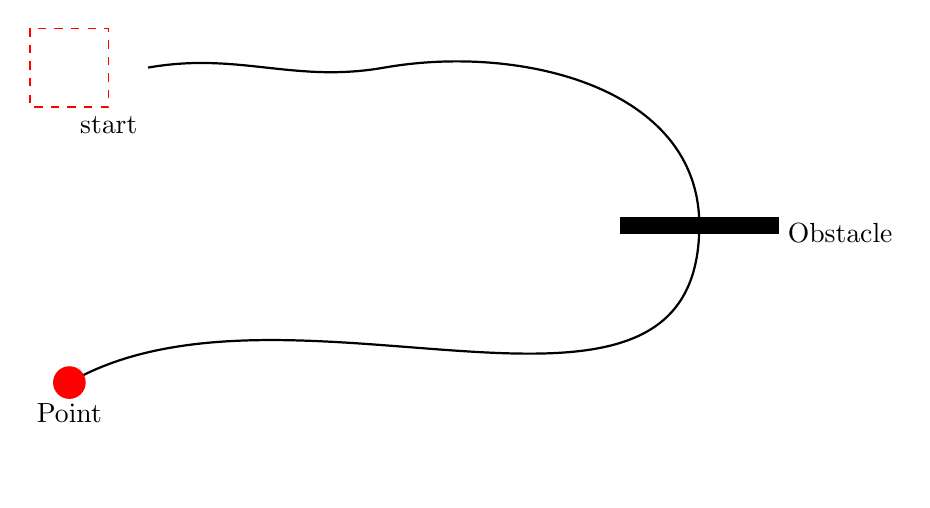
\begin{tikzpicture}
   \draw [red,dashed] (-2.5,2.5) rectangle (-1.5,1.5) node [black,below] {start}; % rectangle
   \draw [thick] (-1,2) % line
   to [out=10,in=190](2,2)
   to [out=10,in=90] (6,0)
   to [out=-90, in=30] (-2, -2);
   \draw [fill] (5,0.1) rectangle (7, -0.1) node [black,right] {Obstacle}; % another rectangle
   \draw [red,fill] (-2, -2) circle [radius=0.2] node [black, below=4] {Point}; % circle
  \end{tikzpicture}
  \caption{Example of tikzpicture}
 \end{center}
\end{figure}

\newpage
\section{Source Code}
\begin{lstlisting}
# Geru.Wrapper/quotes.py

from Geru.Wrapper import session


class Concordance(object):

    @staticmethod
    def get_quotes():
        '''API call to RESTful API  for all quotes.'''
        path = "path to API"
        response = session.get(path)
        return response.json()

    @staticmethod
    def get_quote(ind):
        '''API call to RESTful specific quote'''
        path = "path to API{}".format(ind)
        response = session.get(path)
        return response.json()
\end{lstlisting}

\section{Lists}

\subsection{Unordered List}
\begin{itemize}
 \item One
 \item Two
 \item Three
\end{itemize}

\subsection{Ordered List}
\begin{enumerate}
 \item One
 \item Two
 \item Three
\end{enumerate}

\subsection{Nested List with Numbering / Bullet Manipulation}
\begin{enumerate}[label=$\Gamma$]
 \item One
       \begin{enumerate}
        \item[--] two
        \item[$\ast$] Three
        \item[$\Delta$] Four
       \end{enumerate}
 \item Five
 \item Six
\end{enumerate}

\subsection{Package Enumitem}
\begin{enumerate}[label=(\roman*)]
  \item Roman
  \begin{enumerate}[label=\arabic*]
    \item Arabic
    \begin{enumerate}[label=\alph*]
      \item Alphabet
    \end{enumerate}
  \end{enumerate}
\end{enumerate}

\newpage
\begin{appendix}
 \listoffigures
 \listoftables
\end{appendix}

\end{document}
